\subsection{Ide}

I dette afsnit er der beskrevet en ide til løsningen af den endelige problemformulering. Ideen er resultatet af en diskussion i gruppen, hvor vi kom med ideer til løsninger, og herefter diskuterede fordele og ulemper ved de forskellige ideer. Formålet med afsnittet er at skitsere gruppens bud på den optimale løsning på problemet, og afsnittet er derfor udarbejdet med feedback fra forskellige lampebutikker. I slutningen af afsnittet vil der være en afgrænsning af løsningen som vil danne grundlag for den senere udvikling af en løsning.

Den løsning som gruppen har valgt at arbejde med er, "3D modeller af lamper med interaktion". Som beskrevet i problemanalysen har gruppen valgt at løse problemet når kunder handler på e-butikker. Tanken er derfor at implementere software på en e-butiks hjemmeside med henblik på at løse problemet for kunden. For at skitsere løsningen tager gruppen udgangspunkt i e-butikker der sælger lamper. Skitsen vil benytte sig af URLen "example.com". Dette gøres med henblik på ikke at udstille nogle e-butikker.

\subsubsection{Skitse af løsning}

\begin{figure}[H]
   \centering
   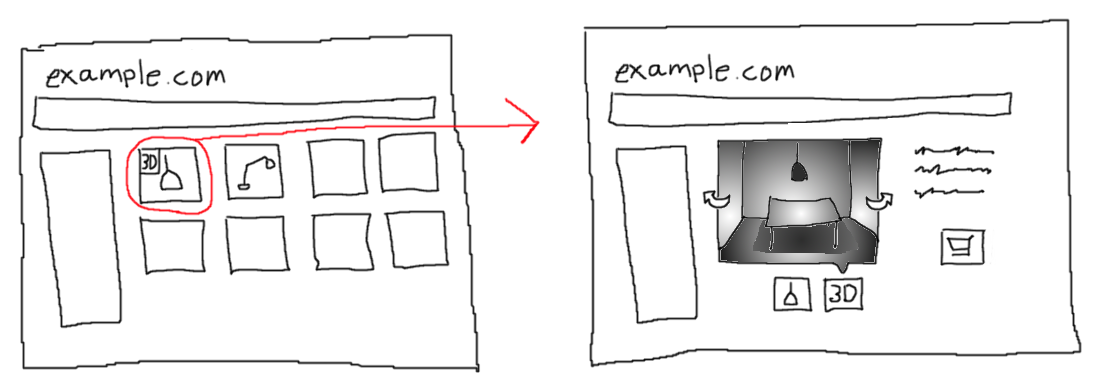
\includegraphics[width=\textwidth]{skitse_til_loesning}
   \caption{Skitse af ide til løsning}.
\end{figure}

På figur 5 er der illusteret en skitse af en e-butik som sælger lamper. Figuren illustrerer hvordan systemet kan integreres på en hjemmeside. Skitse 5a viser et online katalog over e-butikkens udvalg af lamper. Som der fremgår af skitsen vil nogle lamper være markeret med et "3D-ikon" og dette indikerer, at kunden har mulighed for, at se skitsen i 3D. Kunden tilgår 3D-billedet ved at kligge på ikonet. Når kunden trykker på ikonet bliver kunden omdirigeret til en anden menu. Som der fremgår af skitse 5b, så har kunden her mulighed for at se en 3D-model af lampen i et rum. De to pile på skitsen indikerer, at kunden har mulighed for at rotere billedet, og se hvordan belysningen fra lampen er, set fra forskellige vinkler. Ved siden af billedet vil der være mulighed for at læse praktisk information om lampen heriblandt hvem der har produceret lampen. Som en ekstra feature har kunden mulighed for at indtaste en kontekst, beskrevet som en model, ind i programmet og har derefter mulighed for at se hvordan lampen ser ud i den kontekst som brugeren ønsker. Derudover har kunden mulighed for, at justere lampens farvetemperatur (i kelvin), meningen med denne feature er, at kunden har mulighed for at visualisere hvordan forskellige pærer vil se ud i lampen. De forskellige 3D billeder vil ligge til rådighed på en ekstern server og vil derfor ikke gøre e-butikkernes hjemmeside betydeligt langsommere. Derudover er tanken af alle 3D billeder bliver udleveret af producenten af lamperne 

I forbindelse med implementeringen af softwaren på en hjemmeside har der været forskellige ting som skulle overvejes. Da problemet omhandler visualisering af lys fra lamper, har gruppen valgt at fokusere på at lave en løsning hvis primære formål er at generere realistiske 3D-billeder af lamper. Disse billeder vil vise belysningen fra lamper med forskellige pærer. Feature som interaktion og kontekst, har derfor anden priotet. 

Ud fra ovenstående beskrivelse har gruppen derfor valgt at fokusere på at lave et program der gør det muligt for kunden, at visualisere hvordan lys spreder sig fra lamper illustreret igennem realistiske 3D-billeder. Derudover har kunden mulighed for at juserere pærens farvetemperatur, og derved også se hvordan lampens belysning er med forskellige pærer.  


